%introducao.tex

\chapter{Introdução}

Redes sociais vêm crescendo muito nos últimos anos no mundo todo. Além disso, percebe-se que além do crescimento de seu uso, há também a multiplicação de aplicações desse tipo, cada qual focada em um tipo de público específico. 

Uma importante e consolidada forma de incentivo à investigação científica e desenvolvimento tecnológico é a feira de ciências. Feiras de ciências são populares no Brasil e há várias delas. Uma das mais importantes no Brasil é a FEBRACE (Feira Brasileira de Ciências e Engenharia).

  \section{FEBRACE}

  A FEBRACE (Feira Brasileira de Ciências e Engenharia), realizada todos os anos na Escola Politécnica da USP e organizada pelo Nate-LSI (Núcleo de Aprendizagem, Trabalho e Entretenimento do Laboratório de Sistemas Integráveis), é um projeto de ação contínua com o objetivo de estimular a criatividade, a reflexão, o aprofundamento e o raciocínio crítico nas atividades desenvolvidas por estudantes dos Ensinos Fundamental, Médio e Técnico, por meio da indução em realizar projetos investigativos em Ciências, Engenharia e suas aplicações \cite{lopes07}. Além disso, há uma aproximação entre as escolas públicas e privadas das Universidades, criando oportunidades de interação espontânea entre os estudantes e professores das escolas com a comunidade universitária (estudantes, professores, funcionários), para uma melhor compreensão dos papéis das Universidades em Ensino, Pesquisa, Cultura e Extensão. No ano de 2009, a feira chegou a sua 7ª edição.

 A feira conta com a participação de diversas pessoas que possuem diferentes papéis descritos abaixo:

  \begin{description}
    \item[Finalistas] 
        são os estudantes que estão expondo seus projetos na feira;
    \item[Orientadores] 
        são pessoas com idade acima de 21 anos que ajudaram da orientação dos projetos expostos, podendo ser ou não professores;
    \item[Co-orientadores] 
        são pessoas com idade acima de 18 anos que ajudaram da orientação dos projetos expostos, podendo ser ou não professores e
    \item[Acompanhantes] 
        são outras pessoas que vem juntos com os alunos para acompanhá-los durante a feira (por exemplo, pais ou diretores da escola).
  \end{description}

 Na parte do funcionamento da feira em si, a FEBRACE não conta só com os pessoas ligadas ao Laboratório de Sistemas Integráveis da USP para sua organização. Há também uma equipe de apoio, geralmente estudantes de graduação que disponibilizam de seu tempo para participar como voluntários, e uma equipe de avaliadores, que são pessoas que avaliam os projetos expostos na tenda e que devem possuir no mínimo mestrado em uma das áreas de interesse da feira.

A FEBRACE possui sete categorias, que são uma adaptação da tabela de áreas e sub-áreas do conhecimento adotada pela FAPESP (Fundação de Amparo à Pesquisa do Estado de São Paulo):

  \begin{description}
    \item[Ciências Agrárias:] 
        Agronomia, Recursos Florestais e Engenharia Florestal, Engenharia Agrícola, Zootecnia, Medicina Veterinária, Recursos Pesqueiros e Engenharia de Pesca, Ciência e Tecnologia de Alimentos
    \item[Ciências Biológicas:] 
        Biologia Geral, Bioquímica, Genética, Biofísica, Botânica, Farmacologia, Zoologia, Imunologia, Ecologia, Microbiologia, Morfologia, Parasitologia, Fisiologia 	 
    \item[Ciências Exatas e da Terra:] 
        Matemática, Física, Probabilidade e Estatística, Química, Ciência da Computação, Geociências, Astronomia, Oceanografia 
    \item[Ciências Humanas:] 
        Filosofia, Geografia, Sociologia, Psicologia, Antropologia, Educação, Arqueologia, Ciência Política, História, Teologia 
    \item[Ciências da Saúde:] 
        Medicina, Odontologia, Fonoaudiologia, Farmácia, Enfermagem, Fisioterapia e Terapia Ocupacional, Nutrição, Saúde Coletiva, Educação Física
    \item[Ciências Sociais Aplicadas:] 
        Direito, Museologia, Administração, Comunicação, Economia, Serviço Social, Arquitetura e Urbanismo, Economia Doméstica, Planejamento Urbano e Regional, Desenho Industrial, Demografia, Turismo, Ciência da Informação  	 
    \item[Engenharias:] 
        Eletrônica, Sanitária, Eletrotécnica, de Produção, Mecânica, Nuclear, Química, de Transportes, Civil, Naval e Oceânica, de Minas, Aeroespacial, de Materiais e Metalúrgica, Biomédica 
  \end{description}

 A abrangência da FEBRACE pode ser vista através da tabela~\ref{abrangencia}. Segundo estatística da organização da FEBRACE, no ano de 2009, houve a participação de 600 estudantes finalistas, 286 professores orientadores e 241 avaliadores, além de cerca de 30 voluntários no apoio à organização. A feira foi visitada por cerca de 12 mil pessoas nos três dias de exposição. 

\begin{table}[h]
    \begin{center}
        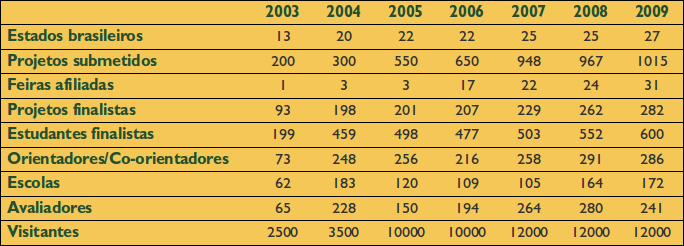
\includegraphics[width=0.8\linewidth]{arquivos/abrangencia.png}
    \end{center}
    \caption{FEBRACE em números}
    \label{abrangencia}
\end{table}

 Outro dado importante sobre a FEBRACE é que esta é uma feira afiliada à Intel ISEF - Feira Internacional de Ciências e Engenharia - realizada anualmente em maio nos EUA em diferentes cidades desse país. A Intel ISEF é a maior feira para estudantes que ainda não chegaram ao nível universitário e participam dessa feira projetos de 50 nações diferentes de todo o mundo.

  \section{Objetivos}

    Dentro do contexto da FEBRACE, o projeto de formatura proposto visa aliar uma aplicação usada atualmente, que é a rede social, e a idéia de feira de ciências, criando assim uma feira virtual de ciências.

    Outro objetivo do projeto é o estudo e a aplicação de alguns conceitos de engenharia de \textit{software}, destacando-se a temática de metódos ágeis de desenvolvimento de \textit{software} e práticas de desenvolvimento web.

  \section{Justificativa}
    A FEBRACE tem um importante papel social no estímulo a aprendizagem de forma criativa e com reflexão em estudantes da educação básica através do desenvolvimento de projetos de ciências e engenharia.

  Com o intuito de aumentar o alcance da Feira, levando-a por mais tempo a mais pessoas, e estimulando a criação de redes entre elas, o presente projeto propõe a criação de uma aplicação Web que possibilite o desenvolvimento e exposição dos projetos na Internet e que ofereça ferramentas que viabilizem maior interação entre os diversos envolvidos na Febrace. Além disso, será mais fácil o envolvimento de pessoas em projetos e a troca de informações entre pessoas interessadas em feiras de ciências, catalizando o papel social da FEBRACE.

  Os impactos descritos acima podem influenciar no interesse de pessoas por uma formação técnica e/ou superior em alguma ciência. Além disso, pode influenciar no espírito de inovação dos envolvidos, podendo estimular avanços significativos em termos tecnológicos e científicos para o país.

  \section{Conceitos Teóricos}

  - Pedagogia de projetos
    - Fernando Almeida (Projetos e Ambientes Inovadores)
    - Lea Fagundes (Aprendizes do Futuro)
    - Paulo Blikstein (Travels in Troy with Freire)

  - Commons Based Peer Production (Free Software, Software social (SS))
    - Benkler (Wealth of Networks - Caps. 1 e 3)
    - Mejias (Nomad's Guide, Learning SS with SS)
